\documentclass[a4paper,12pt]{article}
\usepackage[left=2cm,right=2cm,top=2cm,bottom=2cm]{geometry} % Do ustawień marginesów
\usepackage{booktabs}
\usepackage{longtable}
\usepackage{multicol} % Dla podziału na kolumny
\usepackage{ragged2e} % Dla justowania tekstu
\usepackage{graphicx} % Required for inserting images
\usepackage{float}
\usepackage{caption}
\usepackage{amsmath} % Math formulas
\usepackage{amssymb} % Symbols
\usepackage[svgnames]{xcolor}
\usepackage[colorlinks=true, urlcolor=blue, linkcolor=black, citecolor=orange]{hyperref} % Hyperlinks
\usepackage{polski} % Polish language
\usepackage[utf8]{inputenc} % Text encoding
\usepackage{enumitem} % Pakiet do elastycznego sterowania listami
\usepackage{indentfirst}
\usepackage{array}

\begin{document}

% Górna część strony
\noindent
\begin{minipage}{0.5\textwidth}
    \raggedright
    \textbf{Piotr Durniat} \\
    I rok, Fizyka \\
    Wtorek, 8:00-10:15 \\
    \vspace{0.5cm}
    \vspace{0.5cm}
\end{minipage}%
\begin{minipage}{0.5\textwidth}
    \raggedleft
    18.03.2025 \\
    \vspace{0.5cm} % Dodatkowa linia przerwy
    Prowadząca: \\
    dr Iwona Mróz 
\end{minipage}

% Tytuł ćwiczenia
\vspace{2cm} % Odstęp
\begin{center}
    \LARGE \textbf{Ćwiczenie nr 12} \\[0.5cm]
    \Large \textbf{Laboratoryjny eksperyment symulujący powstawanie kraterów na planetach i księżycach, wskutek uderzeń meteorytów}
\end{center}

% Reszta treści
\vspace{1cm} % Kolejny odstęp
\noindent

\tableofcontents
\newpage


\section{Wstęp teoretyczny}

Celem eksperymentu jest laboratoryjne odwzorowanie procesów powstawania kraterów na powierzchniach ciał niebieskich oraz weryfikacja zależności między energią kinetyczną uderzającego obiektu a wielkością powstałego krateru.

\subsection*{Podstawy fizyczne}

\begin{itemize}
    \item \textbf{Spadek swobodny} -- ruch ciała pod wpływem wyłącznie siły grawitacji, opisany równaniami:
    \begin{align*}
        h &= \frac{1}{2}gt^2 \\
        v &= gt
    \end{align*}
    gdzie $h$ -- wysokość, $v$ -- prędkość, $g$ -- przyspieszenie ziemskie, $t$ -- czas.
    
    \item \textbf{Zasada zachowania energii} -- energia całkowita układu izolowanego pozostaje stała:
    \begin{align*}
        E_p + E_k = \text{const}
    \end{align*}
    Dla kulki spadającej z wysokości $h$ zachodzi przemiana energii potencjalnej w kinetyczną:
    \begin{align*}
        E_p = mgh \rightarrow E_k = \frac{1}{2}mv^2
    \end{align*}
    
    \item \textbf{Zderzenie niesprężyste} -- uderzenie spadającej kulki w piasek powoduje, że część energii kinetycznej zostaje przekształcona w energię deformacji ośrodka.
    
    \item \textbf{Modele tworzenia kraterów} -- rozpatrujemy dwie hipotezy dotyczące zależności między energią kinetyczną uderzającego obiektu a średnicą powstałego krateru:
    \begin{align*}
        \text{Model I:} \quad E_k &\propto D^3 \quad \text{(energia przeznaczona głównie na deformację objętości)} \\
        \text{Model II:} \quad E_k &\propto D^4 \quad \text{(część energii zamieniana na potencjalną materiału wyrzuconego)}
    \end{align*}
\end{itemize}

\subsection*{Metoda logarytmowania}

Aby zlinearyzować zależność potęgową, stosujemy logarytmowanie stronami:
\begin{align*}
    E_k &\propto D^n \\
    E_k &= AD^n \\
    \log(E_k) &= \log(A) + n\log(D)
\end{align*}

Wykreślając zależność $\log(D)$ od $\log(E_k)$ w układzie współrzędnych, otrzymujemy linię prostą o współczynniku kierunkowym $1/n$, co pozwala określić, który z modeli ($n=3$ czy $n=4$) lepiej opisuje eksperyment.

Opracowano na podstawie \cite{lab12manual}.


% \subsection{Analogia do zjawisk astronomicznych}

% W skali astronomicznej, uderzenia meteorytów w powierzchnie planet i księżyców są zderzeniami niesprężystymi o ogromnych energiach. Krater w Arizonie (średnica 1200 m) powstał w wyniku uderzenia meteorytu o masie $M_m \approx 3 \cdot 10^8$ kg z prędkością $v_m \approx 12000$ m/s.

% Przeprowadzany eksperyment stanowi model tego zjawiska w skali laboratoryjnej, umożliwiający ekstrapolację wyników do zjawisk astronomicznych.


\section{Opis doświadczenia}

Doświadczenie polegało na zrzucaniu metalowych kulek o różnych masach z różnych wysokości na powierzchnię suchego, drobnoziarnistego piasku. Kulki były upuszczane swobodnie, bez nadawania im prędkości początkowej. Po każdym uderzeniu mierzono średnicę powstałego krateru.

Wykorzystano trzy kulki o różnych masach i średnicach (tabela \ref{tab:kulki}). Pomiary wykonywano dla wysokości od 0,25 m do 2,0 m. Dla każdej kombinacji kulki i wysokości wykonano po 5 pomiarów średnicy krateru w celu zminimalizowania błędów przypadkowych.

Piasek przed każdą serią pomiarów był wyrównywany i delikatnie ubijany w celu zapewnienia jednorodnych warunków początkowych. Średnicę kraterów mierzono przy pomocy suwmiarki z dokładnością do 0,001 cm.



\section{Opracowanie wyników pomiarów}

\subsection{Tabele pomiarowe}

\begin{center}
    \begin{tabular}{|c|c|c|}
        \hline
        Rodzaj kulki & Masa [g] & Średnica [cm] \\
        \hline
        Mała & 4,1 & 1,000 \\
        Średnia & 14,0 & 1,500 \\
        Duża & 31,7 & 2,000 \\
        \hline
    \end{tabular}
    \captionof{table}{Parametry kulek używanych w doświadczeniu}
    \label{tab:kulki}
\end{center}

\begin{center}
    \begin{tabular}{|c|c|c|c|c|c|}
        \hline
        Wysokość [m] & 0,25 & 0,5 & 1,0 & 1,5 & 2,0 \\
        \hline
        Nr pomiaru & \multicolumn{5}{c|}{Średnica krateru [cm]} \\
        \hline
        1 & 3,170 & 3,760 & 4,310 & 4,625 & 4,760 \\
        2 & 2,880 & 3,845 & 3,910 & 4,510 & 4,875 \\
        3 & 2,870 & 3,810 & 4,220 & 4,430 & 4,365 \\
        4 & 3,635 & 3,580 & 4,350 & 4,615 & 4,575 \\
        5 & 2,965 & 3,665 & 4,060 & 4,550 & 4,880 \\
        \hline
    \end{tabular}
    \captionof{table}{Pomiary średnicy kraterów dla małej kulki}
    \label{tab:kratery_mala}
\end{center}

\begin{center}
    \begin{tabular}{|c|c|c|c|c|}
        \hline
        Wysokość [m] & 0,5 & 1,0 & 1,5 & 2,0 \\
        \hline
        Nr pomiaru & \multicolumn{4}{c|}{Średnica krateru [cm]} \\
        \hline
        1 & 4,760 & 5,265 & 6,210 & 6,995 \\
        2 & 4,750 & 5,270 & 6,055 & 6,890 \\
        3 & 4,920 & 5,380 & 6,355 & 6,885 \\
        4 & 4,930 & 5,800 & 6,155 & 6,610 \\
        5 & 5,120 & 5,600 & 6,225 & 6,775 \\
        \hline
    \end{tabular}
    \captionof{table}{Pomiary średnicy kraterów dla średniej kulki}
    \label{tab:kratery_srednia}
\end{center}

\begin{center}
    \begin{tabular}{|c|c|c|}
        \hline
        Wysokość [m] & 1,5 & 2,0 \\
        \hline
        Nr pomiaru & \multicolumn{2}{c|}{Średnica krateru [cm]} \\
        \hline
        1 & 7,310 & 7,980 \\
        2 & 7,440 & 7,525 \\
        3 & 7,460 & 8,035 \\
        4 & 7,375 & 8,040 \\
        5 & 7,175 & 7,700 \\
        \hline
    \end{tabular}
    \captionof{table}{Pomiary średnicy kraterów dla dużej kulki}
    \label{tab:kratery_duza}
\end{center}

% --- Średnia średnica krateru ---

\subsection{Średnia średnica krateru, energia potencjalna kulki i logarytmy obu wielkości}


Dla każdej kombinacji wysokości i rozmiaru kulki wykonano po pięć pomiarów średnicy powstałego krateru. Średnia średnica krateru $\overline{D}$ została obliczona jako średnia arytmetyczna z tych pomiarów według wzoru:

\[ \overline{D} = \frac{1}{5}\sum_{i=1}^{5} D_i \]

Energia potencjalna kulki została obliczona ze wzoru $E_p = mgh$, gdzie:
\begin{itemize}
    \item $m$ - masa kulki [kg]
    \item $g$ - przyspieszenie ziemskie [$\frac{m}{s^2}$]
    \item $h$ - wysokość z jakiej upuszczono kulkę [m]
\end{itemize}

Następnie, w celu zlinearyzowania zależności potęgowej między energią a średnicą krateru, obliczono logarytmy dziesiętne obu wielkości:

\[ \log_{10}(\overline{D}) \quad \text{oraz} \quad \log_{10}(E_p) \]

Wartości te zostały wykorzystane do sporządzenia wykresu w układzie podwójnie logarytmicznym, co pozwoli na określenie wykładnika potęgowego badanej zależności.


\begin{center}
    \begin{tabular}{|c|c|c|c|c|c|}
        \hline
        Wysokość [m] & 0,2 & 0,5 & 1,0 & 1,5 & 2,0 \\
        \hline
        $\overline{D}$ [m] & 0,03104 & 0,03732 & 0,04170 & 0,04546 & 0,04691 \\
        \hline
        $E_p$ [J] & 0,0101 & 0,0201 & 0,0402 & 0,0603 & 0,0804 \\
        \hline
        $\log_{10}(\overline{D})$ & -1,5081 & -1,4281 & -1,3799 & -1,3424 & -1,3287 \\
        \hline
        $\log_{10}(E_p)$ & -1,9976 & -1,6966 & -1,3955 & -1,2195 & -1,0945 \\
        \hline
    \end{tabular}
    \captionof{table}{Wyniki pomiarów dla małej kulki}
    \label{tab:wyniki_mala}
\end{center}

\begin{center}
    \begin{tabular}{|c|c|c|c|c|}
        \hline
        Wysokość [m] & 0,5 & 1,0 & 1,5 & 2,0 \\
        \hline
        $\overline{D}$ [m] & 0,04896 & 0,05463 & 0,06200 & 0,06831 \\
        \hline
        $E_p$ [J] & 0,0687 & 0,1373 & 0,2060 & 0,2747 \\
        \hline
        $\log_{10}(\overline{D})$ & -1,3102 & -1,2626 & -1,2076 & -1,1655 \\
        \hline
        $\log_{10}(E_p)$ & -1,1632 & -0,8622 & -0,6861 & -0,5612 \\
        \hline
    \end{tabular}
    \captionof{table}{Wyniki pomiarów dla średniej kulki}
    \label{tab:wyniki_srednia}
\end{center}

\begin{center}
    \begin{tabular}{|c|c|c|}
        \hline
        Wysokość [m] & 1,5 & 2,0 \\
        \hline
        $\overline{D}$ [m] & 0,07352 & 0,07856 \\
        \hline
        $E_p$ [J] & 0,4665 & 0,6220 \\
        \hline
        $\log_{10}(\overline{D})$ & -1,1336 & -1,1048 \\
        \hline
        $\log_{10}(E_p)$ & -0,3312 & -0,2062 \\
        \hline
    \end{tabular}
    \captionof{table}{Wyniki pomiarów dla dużej kulki}
    \label{tab:wyniki_duza}
\end{center}

\subsection{Wykres zależności średnicy krateru od energii potencjalnej}

Za pomocą języka Python i biblioteki matplotlib został wygenerowany wykres zależności energii potencjalnej od średnicy krateru. Wykres został sporządzony w układzie podwójnie logarytmicznym i zamieszczony na rysunku \ref{rys:energia_od_srednicy}.

\subsection{Regresja liniowa - wyznaczenie wykładnika potęgi}

Do analizy zależności między energią potencjalną a średnicą krateru wykorzystano regresję liniową w skali logarytmicznej. Dane zostały przetworzone przy użyciu języka Python i biblioteki NumPy.

Regresja liniowa została wykonana na zlogarytmowanych wartościach energii potencjalnej ($\log_{10}(E_p)$) i średnicy krateru ($\log_{10}(D)$). Wykorzystano funkcję \texttt{numpy.polyfit}, która dopasowuje wielomian (w tym przypadku pierwszego stopnia) do danych metodą najmniejszych kwadratów.


Otrzymana prosta ma postać:
\[ \log_{10}(E_p) = a\log_{10}(D) + b \]

gdzie:
\begin{itemize}
    \item $a = 4,37$ - współczynnik kierunkowy prostej
    \item $b = 4,61$ - wyraz wolny
\end{itemize}

Po przekształceniu wzoru na postać potęgową otrzymujemy:
\[ E_p = 10^{4,61} \cdot D^{4,37} \approx 4,07 \cdot 10^4 \cdot D^{4,37} \]
\section{Ekstrapolacja wyników}

\subsection{Energia potencjalna na podstawie obliczonej zależności}

Korzystając z otrzymanego wcześniej wzoru:
\[
E_p = 10^{4,61} \cdot D^{4,37} \approx 4,07 \cdot 10^4 \cdot D^{4,37}
\]

Dla średnicy krateru \( D = 1200 \, \text{m} \) otrzymujemy:
\begin{align*}
E_p &\approx 4,07 \cdot 10^4 \cdot (1200)^{4,37} \\
&\approx 4,07 \cdot 10^4 \cdot 2,22 \cdot 10^{12} \\
&\approx 9,05 \cdot 10^{16} \, \text{J}
\end{align*}

\subsection{Energia kinetyczna na podstawie danych historycznych}

Energię kinetyczną meteorytu obliczamy ze wzoru:
\[
E_k = \frac{1}{2} m v^2
\]

Dla danych:
\begin{itemize}
    \item masa meteorytu: \( m = 3 \cdot 10^8 \) kg
    \item prędkość meteorytu: \( v = 12000 \) m/s
\end{itemize}

otrzymujemy:
\begin{align*}
E_k &= \frac{1}{2} \cdot (3 \cdot 10^8) \cdot (12000)^2 \\
&= 1,5 \cdot 10^8 \cdot 1,44 \cdot 10^8 \\
&= 2,16 \cdot 10^{16} \text{ J}
\end{align*}

\section{Ocena niepewności pomiaru}

Dla wszystkich przyrządów pomiarowych niepewność standardową typu B obliczono według wzoru:

\begin{equation}
    \label{eq:unc_B}
    u_B(x) = \frac{\Delta x}{\sqrt{3}}
\end{equation}
gdzie $\Delta x$ oznacza dokładność wzorcowania przyrządu pomiarowego.

\subsection{Niepewność masy kulek}
Masy kulek zapisane w tabeli \ref{tab:kulki} zmierzono za pomocą wagi analitycznej o dokładności wzorcowania $\Delta m = 0,1 \, \text{g}$. 

Korzystając ze wzoru \eqref{eq:unc_B}, otrzymujemy:

$$
u_B(m) = 5,8 \cdot 10^{-5} \, \text{m}
$$

\subsection{Niepewność średnicy kulek}
Do pomiaru średnicy kulek przedstawionych w tabeli \ref{tab:kulki} wykorzystano suwmiarkę o dokładności wzorcowania $\Delta d = 0,05 \, \text{mm}$. 

Zgodnie ze wzorem \eqref{eq:unc_B}:
\[
u_B(d) = 2,9 \cdot 10^{-5} \, \text{m}
\]

\subsection{Niepewność wysokości}
Do pomiaru wysokości została użyta miara metrowa o dokładności wzorcowania $\Delta h = 0,01 \, \text{m}$. 

Stosując wzór \eqref{eq:unc_B}:
\[
u_B(h) = 0,0058 \, \text{m}
\]

\subsection{Niepewność średnicy kraterów}

Do obliczenia odchylenia standardowego średnicy kraterów $u_A(D)$ użyto poniższego wzoru:

\[
u_A(D) = \sqrt{\frac{1}{n-1} \sum_{i=1}^{n} (D_i - \bar{D})^2}
\]

gdzie:

\begin{itemize}
    \item \( D_i \) to wartość pojedynczego pomiaru,
    \item \( \bar{D} \) to średnia z pomiarów,
    \item \( n \) to liczba pomiarów.
\end{itemize}

Otrzmane wyniki przedstawia tabela \ref{tab:odchylenia_standardowe_srednicy}.

\begin{table}[H]
\centering
\begin{tabular}{|c|c|c|c|}
\hline
\textbf{Wysokość $h$ [m]} & \multicolumn{3}{c|}{\textbf{$u_A(D)$ [m]}} \\
\hline
& \textbf{Mała kulka} & \textbf{Średnia kulka} & \textbf{Duża kulka} \\
\hline
0,25 & 0,0032 & - & - \\
 \hline
 0,5  & 0,0011 & 0,0015 & - \\
 \hline
 1,0  & 0,0018 & 0,0023 & - \\
 \hline
 1,5  & 0,00080 & 0,0011 & 0,0012 \\
 \hline
 2,0  & 0,0022 & 0,0015 & 0,0023 \\
\hline
\end{tabular}
\caption{Odchylenie standardowe średnicy kraterów dla poszczególnych kulek}
\label{tab:odchylenia_standardowe_srednicy}
\end{table}

Następnie obliczono niepewność typu B średnicy kraterów $u_B(D)$ na podstawie wzoru \eqref{eq:unc_B} i otrzymano wartość: 

$$
u_B(D) = 0,029 \, \text{m}
$$

Następnie obliczono niepewność całkowitą średnicy kraterów $u_c(D)$ na podstawie wzoru:

\[
u_c(D) = \sqrt{u_A(D)^2 + u_B(D)^2}
\]

Otrzymane wyniki przedstawia tabela \ref{tab:niepewnosc_calkowita_srednicy}.

\begin{table}[H]
\centering
\begin{tabular}{|c|c|c|c|}
\hline
\textbf{Wysokość $h$ [m]} & \multicolumn{3}{c|}{\textbf{$u_c(D)$ [m]}} \\
\hline
& \textbf{Mała kulka} & \textbf{Średnia kulka} & \textbf{Duża kulka} \\
\hline
0,25 & 0,0032 & - & - \\
\hline
0,5  & 0,0011 & 0,0015 & - \\
\hline
1,0  & 0,0018 & 0,0023 & - \\
\hline
1,5  & 0,00080 & 0,0011 & 0,0012 \\
\hline
2,0  & 0,0022 & 0,0015 & 0,0023 \\
\hline
\end{tabular}
\caption{Niepewność całkowita średnicy kraterów dla wszystkich kulek}
\label{tab:niepewnosc_calkowita_srednicy}
\end{table}

Przykładowe obliczenie dla małej kulki przy wysokości $h=1,5\,\text{m}$:

\begin{align*}
u_A(D) &= \sqrt{\begin{gathered}
    \frac{1}{4} [(4,625 - 4,546)^2 + (4,510 - 4,546)^2 + \\
    (4,430 - 4,546)^2 + (4,615 - 4,546)^2 + (4,550 - 4,546)^2]
\end{gathered}} \\
&= 0,00080\,\text{m}
\end{align*}

$$
u_B(D) = \frac{0,05}{\sqrt{3}} = 0,029\,\text{m} \\[1em]
$$

$$
u_c(D) = \sqrt{(0,00080)^2 + (0,029)^2} = 0,029\,\text{m}
$$




\subsection{Niepewność energii potencjalnej}

korzystając z prawa przenoszenia niepewności otrzymano:


$$
u_c(E) = \sqrt{\left(\frac{\partial E}{\partial m}\right)^2 u_c(m)^2 + \left(\frac{\partial E}{\partial h}\right)^2 u_c(h)^2}
$$

Po podstawieniu wzoru na energię potencjalną $E = mgh$ otrzymano:

\begin{align*}
u_c(E) = \sqrt{g^2h^2 u_c(m)^2 + g^2m^2 u_c(h)^2} = \\
= g\sqrt{h^2u_c(m)^2 + m^2u_c(h)^2}
\end{align*}

Dla wszystkich kulek i wszystkich wysokości otrzymano wartości niepewności energii potencjalnej przedstawione w tabeli \ref{tab:niepewnosc_calkowita_energii}.

\begin{table}[H]
\centering
\begin{tabular}{|c|c|c|c|}
\hline
\textbf{Wysokość $h$ [m]} & \multicolumn{3}{c|}{\textbf{$u_c(E)$ [J]}} \\
\hline
& \textbf{Mała kulka} & \textbf{Średnia kulka} & \textbf{Duża kulka} \\
\hline
0,25 & 0,0024 & - & - \\
\hline
0,5 & 0,0024 & 0,0083 & - \\
\hline
1,0 & 0,0025 & 0,0083 & - \\
\hline
1,5 & 0,0026 & 0,0083 & 0,019 \\
\hline
2,0 & 0,0027 & 0,0083 & 0,019 \\
\hline
\end{tabular}
\caption{Niepewność całkowita energii potencjalnej dla wszystkich kulek}
\label{tab:niepewnosc_calkowita_energii}
\end{table}

Przykładowe obliczenia niepewności energii potencjalnej dla małej kulki (o masie 4,1 g) na wysokości $h = 0,25$ m:

$$
u_c(E) = 9,81 \sqrt{(0,25)^2 \cdot (6,00\cdot10^{-5})^2 + (0,0041)^2 \cdot (0,0058)^2} = 0,0024 \text{ J}
$$


\subsection{Niepewność pomiarowa współczynników prostej regresji liniowej}

Niepewności pomiarowe dla wyznaczonej prostej regresji liniowej $y = ax + b$ obliczono na podstawie odchylenia standardowego reszt $s_y$ oraz rozkładu punktów pomiarowych wzdłuż osi $x$, korzystając z następujących wzorów:

\[
s_y = \sqrt{\frac{\sum_{i=1}^{n} (y_i - \hat{y}_i)^2}{n-2}}
\]

\[
u_a = s_y \sqrt{\frac{n}{n \sum x_i^2 - \left( \sum x_i \right)^2}}
\]

\[
u_b = s_y \sqrt{\frac{\sum x_i^2}{n \sum x_i^2 - \left( \sum x_i \right)^2}}
\]

gdzie $x_i$ to wartości zmiennej niezależnej, $y_i$ to wartości zmierzone, $\hat{y}_i$ to wartości przewidywane przez model regresji, a $n$ to liczba punktów pomiarowych. Dzielnik $n-2$ wynika z faktu, że model regresji liniowej ma dwa parametry ($a$ i $b$).


Obliczone wartości niepewności dla współczynników prostej regresji wyniosły odpowiednio:

\begin{itemize}
    \item $u_a = 0,14$
    \item $u_b = 0,018$
\end{itemize}

\newpage

\section{Wnioski}

Wykładnik potęgi $a = 4,37(14)$ sugeruje, że zależność między energią potencjalną a średnicą krateru jest bliższa modelowi II ($E_k \propto D^4$) niż modelowi I ($E_k \propto D^3$).

Ekstrapolując otrzymaną zależność do skali astronomicznej, możemy porównać przewidywania naszego modelu z rzeczywistymi danymi. Dla krateru w Arizonie o średnicy 1200 m i meteorytu o masie $3\cdot10^8$ kg i prędkości $12000$ m/s, energia kinetyczna meteorytu wynosiła:

\begin{itemize}
    \item Według danych historycznych: $E_k = \frac{1}{2}mv^2 = 2,16\cdot10^{16} \text{ J}$
    \item Według naszego modelu ($E_k \propto D^{4,37}$): $E_k = 9.05\cdot10^{16} \text{ J}$
\end{itemize}

Wartość według naszego modelu jest o $76\%$ większa od wartości historycznej. Jest to stosunkowo dobra zgodność biorąc pod uwagę, że ekstrapolujemy wyniki z eksperymentu laboratoryjnego (skala centymetrów) do zjawiska astronomicznego (skala kilometrów).


\section{Wykresy}

\begin{figure}[H]
    \centering
    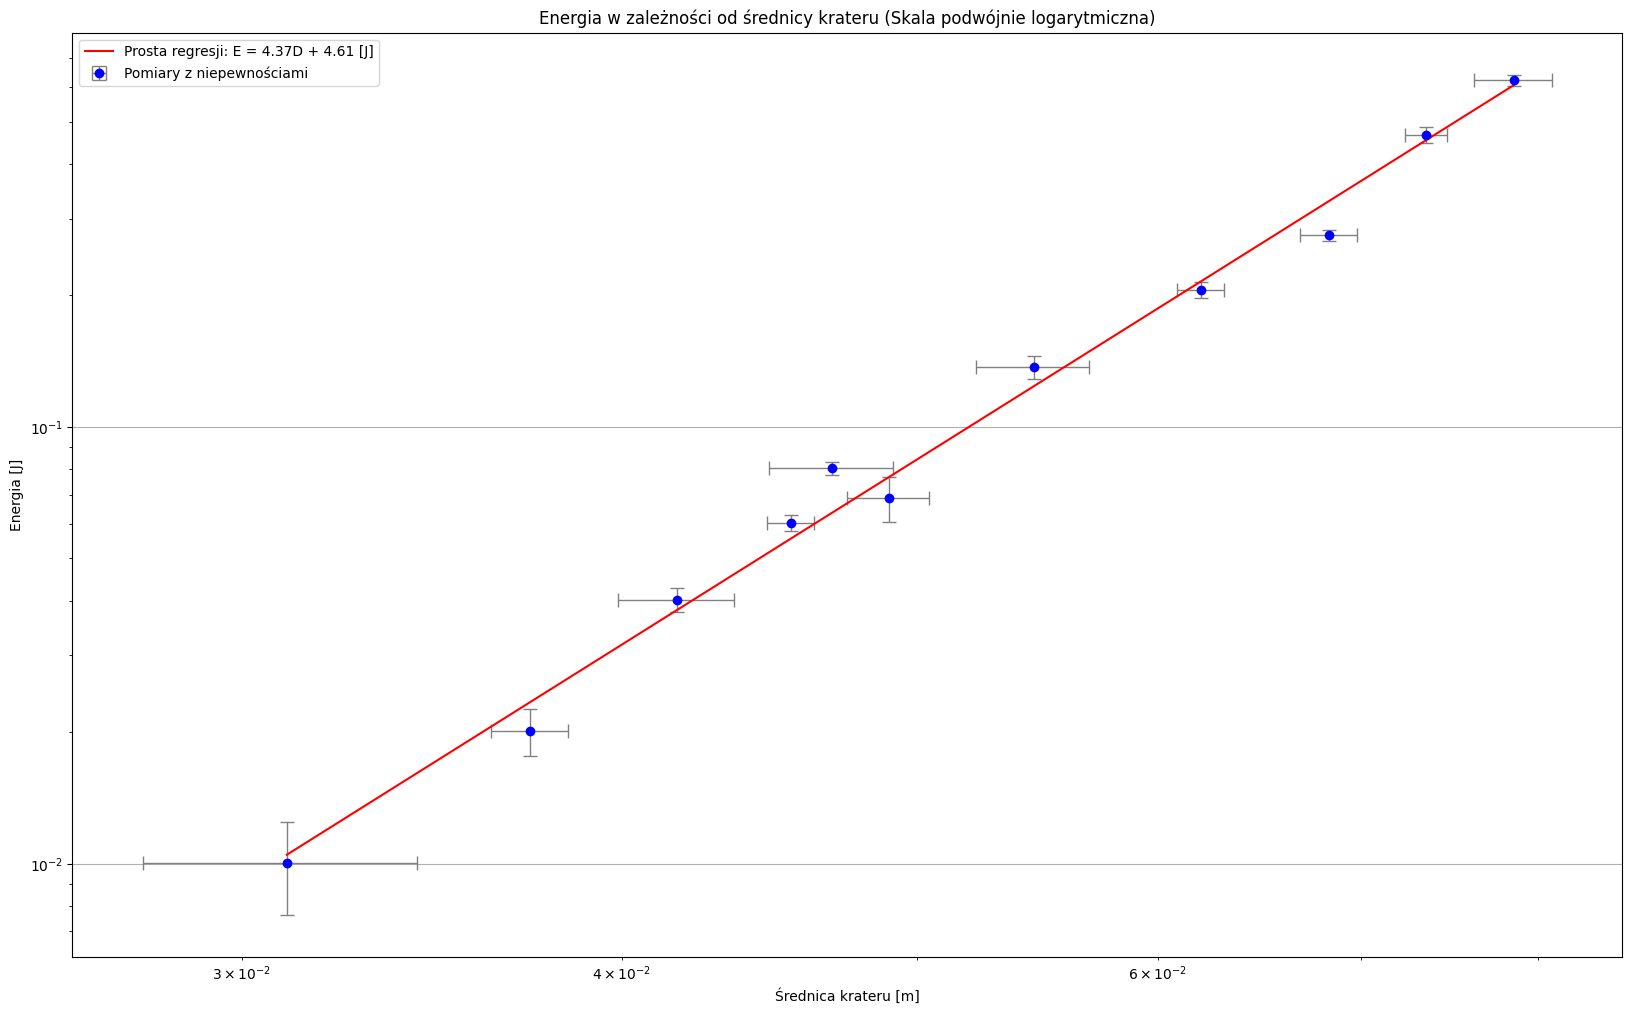
\includegraphics[angle=90,height=0.90\textheight]{energia_od_srednicy.png}
    \caption{Wykres zależności energii potencjalnej od średnicy krateru (Źródło: opracowanie własne)}
    \label{rys:energia_od_srednicy}
\end{figure}

\bibliographystyle{plain}
\bibliography{bibliography}


\end{document}
